% ============================================================================
% Session 9: Continuous-time heterogeneous agents (Padova, September 2026)
% Extracted from the Geneva 2026 CT-HA theory and numerics decks; see _src_CT_*.tex.
% University of Padova, 23-24 September 2026
% April 20--23 & May 4--7, 2026
% Duration: 75 minutes
% ============================================================================

\documentclass[aspectratio=169,11pt]{beamer}

% ---------- Theme and colors ----------
\usecolortheme{dove}
\setbeamertemplate{navigation symbols}{}
\setbeamertemplate{footline}{%
  \hfill\usebeamerfont{page number in head/foot}%
  \usebeamercolor[fg]{normal text}%
  \insertframenumber\,/\,\inserttotalframenumber\kern1em\vskip4pt}
\setbeamerfont{frametitle}{size=\huge}

% ---------- Packages ----------
\usepackage[utf8]{inputenc}
\usepackage[T1]{fontenc}
\usepackage{amsmath,amssymb,amsfonts}
\usepackage{bm}
\usepackage{graphicx}
\usepackage{tikz}
\usetikzlibrary{shapes,arrows.meta,positioning,calc,fit,backgrounds,patterns,decorations.pathreplacing}
\usepackage{pgfplots}
\pgfplotsset{compat=1.18}
\usepackage{booktabs}
\usepackage{hyperref}
\usepackage{multicol}
\usepackage{xcolor}
\usepackage{algorithm}
\usepackage{algorithmic}
\usepackage{listings}
\usepackage{pifont}

% ---------- Listings style for Python ----------
\lstset{
    language=Python,
    basicstyle=\footnotesize\ttfamily,
    keywordstyle=\color{uzhblue}\bfseries,
    commentstyle=\color{uzhgreydark}\itshape,
    stringstyle=\color{darkgreen},
    showstringspaces=false,
    breaklines=true,
    frame=none,
    xleftmargin=0pt,
    aboveskip=2pt,
    belowskip=2pt,
    escapeinside={(*@}{@*)},
}

% ---------- Custom colors ----------
\definecolor{uzhblue}{rgb}{0,0,0.5}
\definecolor{uzhgreylight}{RGB}{236,238,241}
\definecolor{uzhgreydark}{RGB}{81,86,94}
\definecolor{harvardcrimson}{RGB}{153,0,0}
\definecolor{unil@blue}{RGB}{0,140,204}
\definecolor{unil@black}{RGB}{35,31,32}
\definecolor{darkgreen}{RGB}{0,100,0}
\definecolor{darkred}{RGB}{139,0,0}
\definecolor{softblue}{RGB}{70,130,180}
\definecolor{softorange}{RGB}{230,159,0}
\definecolor{softgreen}{RGB}{0,158,115}

% ---------- Set beamer colors ----------
\setbeamercolor{frametitle}{bg=uzhgreylight, fg=uzhblue}
\setbeamercolor{title}{fg=uzhblue}
\setbeamercolor{structure}{fg=uzhblue}
\setbeamercolor{block title}{bg=unil@blue, fg=white}
\setbeamercolor{block body}{bg=uzhgreylight}
\setbeamercolor{block title alerted}{bg=darkred,fg=white}
\setbeamercolor{block body alerted}{bg=red!5}
\setbeamercolor{block title example}{bg=darkgreen,fg=white}
\setbeamercolor{block body example}{bg=green!5}
\setbeamercolor{item}{fg=unil@black}
\setbeamercolor{normal text}{fg=unil@black}

% ---------- Emphasis and hyperlinks ----------
\newcommand{\emphc}[1]{\textcolor{harvardcrimson}{#1}}
\hypersetup{colorlinks,linkcolor=harvardcrimson,urlcolor=harvardcrimson}

% ---------- Reduce vertical spacing ----------
\setlength{\parskip}{0pt}

% ---------- Math commands ----------
\newcommand{\R}{\mathbb{R}}
\newcommand{\E}[1]{\mathbb{E}\!\left[#1\right]}
\DeclareMathOperator*{\argmin}{arg\,min}
\DeclareMathOperator*{\argmax}{arg\,max}
\newcommand{\ud}{\,\mathrm{d}}
\newcommand{\ubar}[1]{\underline{#1}}

% ---------- Title ----------
\title[Continuous time -- Padova 2026]%
{Deep Learning for Solving Dynamic Models}
\subtitle{Session 9 --- Continuous-time heterogeneous agents: HJB, KFE, and PINNs}
\author{Simon Scheidegger}
\institute[HEC Lausanne]{HEC, University of Lausanne}
\date{University of Padova\\September 24, 2026}

\begin{document}

% --- Title ---
{\setbeamercolor{background canvas}{bg=uzhgreylight}
\begin{frame}
\titlepage
\vspace{-0.4cm}
\begin{center}
{\footnotesize Based on: Achdou, Han, Lasry, Lions \& Moll (2022), \emph{Rev.\ Econ.\ Stud.}\ 89(1), 45--86.}\\[2pt]
{\footnotesize Gu, Lauri\`ere, Merkel \& Payne (2024), ``Global Solutions to Master Equations.'' arXiv:2406.13726.}
\end{center}
\end{frame}
}

\begin{frame}{Roadmap of This Session (40 min)}
\begin{enumerate}\itemsep6pt
  \item \textbf{Why continuous time} --- what the reformulation buys us (5 min)
  \item \textbf{The HJB--KFE system} --- individual optimization plus the cross-sectional
        distribution; Aiyagari mapped operator by operator (20 min)
  \item \textbf{Numerics} --- upwind finite differences versus a PINN on the identical
        problem, and when each stops being viable (15 min)
\end{enumerate}
\vspace{6pt}
\begin{block}{Where this sits}
Session 8 turned a PDE residual into a loss. Here that machinery meets the
canonical heterogeneous-agent model, and we compare it against the classical
finite-difference benchmark.
\end{block}
\end{frame}

\section{Why Continuous Time}
\begin{frame}{Why Continuous Time?}
\begin{columns}[T]
\column{0.55\textwidth}
\textbf{Advantages of continuous-time formulation:}
\begin{itemize}\itemsep2pt
    \item \emphc{Analytical tractability}: Ito calculus provides closed-form FOCs
    \item \emphc{Clean separation}: HJB (backward) $\leftrightarrow$ KFE (forward)
    \item \emphc{Powerful numerical methods}: finite differences, PINNs
    \item \emphc{No expectations operator}: replaced by differential operators
    \item \emphc{Connection to mean field games} (Lasry \& Lions, 2007)
\end{itemize}

\column{0.42\textwidth}
\begin{block}{Key References}
\small
\begin{itemize}\itemsep2pt
    \item Achdou, Han, Lasry, Lions \& Moll (2022), \emph{REStud}
    \item Kaplan, Moll \& Violante (2018), \emph{AER}
    \item Moll lecture notes:\\ \url{benjaminmoll.com/lectures/}
\end{itemize}
\end{block}

\vspace{0.3em}
\begin{alertblock}{\small Discrete $\to$ Continuous}
\small
Day 4 (DEQNs, Young's method) used \emph{discrete time}.\\
Today: \emph{continuous time} $\Rightarrow$ PDEs.
\end{alertblock}
\end{columns}
\end{frame}

\begin{frame}{The Aiyagari--Bewley--Huggett Framework}
\small
\begin{itemize}\itemsep2pt
    \item Benchmark models in ``quantitative'' macroeconomics:
    \begin{itemize}\itemsep2pt
        \item \textbf{Bewley} (1980, 1983): precautionary saving with borrowing constraints
        \item \textbf{Huggett} (1993, \emph{JEDC}): endowment economy, risk-free rate determination
        \item \textbf{Aiyagari} (1994, \emph{QJE}): production economy, general equilibrium
        \item \textbf{Krusell \& Smith} (1998, \emph{JPE}): adds aggregate TFP shocks
    \end{itemize}
    \item Core mechanism: \emphc{idiosyncratic labor income risk} is \emphc{uninsurable}
    \begin{itemize}
        \item Households want to borrow when income is low $\to$ borrowing limits prevent this
        \item Instead, households accumulate assets as \emphc{precautionary savings}
    \end{itemize}
    \item These are building blocks for \emphc{HANK} models (Kaplan, Moll \& Violante, 2018)
    \begin{itemize}
        \item Heterogeneous Agent New Keynesian: monetary/fiscal policy with inequality
    \end{itemize}
\end{itemize}
\end{frame}


\section{The HJB--KFE System}
\begin{frame}{It\^o Processes and SDEs}
\small
\begin{block}{General It\^o Process}
A stochastic process $X_t$ follows an \emphc{It\^o process} if:
\vspace{-0.3em}
\[
\boxed{dX_t = \mu(X_t, t)\ud t + \sigma(X_t, t)\ud B_t}
\]
\vspace{-0.5em}
\begin{itemize}\itemsep1pt
    \item $\mu(X_t, t)$: \emphc{drift} (deterministic trend)
    \item $\sigma(X_t, t)$: \emphc{diffusion coefficient} (volatility / noise intensity)
    \item $B_t$: standard Brownian motion
\end{itemize}
\end{block}

\vspace{0.1em}
\textbf{Important examples:}
\begin{columns}[T]
\column{0.48\textwidth}
\begin{exampleblock}{\small Geometric Brownian Motion (GBM)}
$dS_t = \mu S_t \ud t + \sigma S_t \ud B_t$\\[2pt]
{\small Used for: stock prices, GDP}
\end{exampleblock}

\column{0.48\textwidth}
\begin{exampleblock}{\small Ornstein--Uhlenbeck (OU) Process}
$dZ_t = \eta(\bar{Z} - Z_t)\ud t + \sigma \ud B_t$\\[2pt]
{\small Used for: productivity, interest rates}
\end{exampleblock}
\end{columns}
\end{frame}

\begin{frame}{What Is the Kolmogorov Forward Equation?}
\small
\begin{columns}[T]
\column{0.58\textwidth}
The \emphc{Kolmogorov forward equation} (KFE), also known as the \emphc{Fokker--Planck equation}, describes how the \textbf{probability density} of a stochastic process evolves over time.

\vspace{0.3em}
\textbf{Origin}: physics and applied mathematics.
\begin{itemize}\itemsep2pt
    \item \textbf{A.N.\ Kolmogorov} (1931): general theory of continuous Markov processes
    \item \textbf{A.D.\ Fokker} (1914) \& \textbf{M.\ Planck} (1917): diffusion of particles
    \item Applications: heat conduction, fluid dynamics, plasma physics, chemical kinetics, population genetics, neuroscience, \ldots
\end{itemize}

\column{0.38\textwidth}
\begin{center}
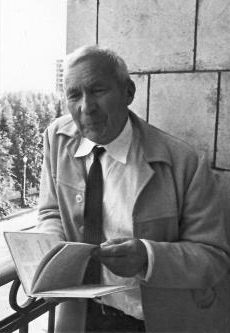
\includegraphics[width=0.78\linewidth,height=0.34\textheight,keepaspectratio]{images/kolmogorov.jpg}\\[-2pt]
{\tiny A.N.\ Kolmogorov, Wikimedia Commons}
\end{center}
\end{columns}

\vspace{0.1em}
{\small \textbf{Key idea}: micro dynamics (drift + noise) $\Rightarrow$ macro density law of motion.}
\end{frame}

\begin{frame}{The KFE: General It\^o Diffusion}
\small
For $dX_t = \mu(X_t)\ud t + \sigma(X_t)\ud B_t$ with \emphc{state-dependent} drift and diffusion,
the density $g(x,t)$ satisfies the \textbf{general KFE}:

\begin{block}{Kolmogorov Forward / Fokker--Planck Equation}
\vspace{-0.5em}
\[
\boxed{\frac{\partial g}{\partial t}(x,t) = -\frac{\partial}{\partial x}\big[\mu(x)\,g(x,t)\big] + \frac{1}{2}\frac{\partial^2}{\partial x^2}\big[\sigma(x)^2\,g(x,t)\big]}
\]
\vspace{-0.5em}
\end{block}

\textbf{Important}: when $\sigma$ depends on $x$, it enters \emph{inside} the second derivative:
$\frac{1}{2}\partial_{xx}\!\left[\sigma(x)^2 g\right] \;\neq\; \frac{\sigma(x)^2}{2}\partial_{xx}g$

In \emphc{divergence form}: $\partial_t g = -\partial_x\underbrace{\left[\mu(x)g - \frac{1}{2}\partial_x(\sigma^2 g)\right]}_{=:\text{probability flux } J(x,t)}$
\quad Conservation law: $\partial_t g + \partial_x J = 0$.
\end{frame}

\begin{frame}{KFE in Economics: The Wealth Distribution}
\small
\textbf{Setup}: Agent $i$ has wealth $a_t^i$ and income state $n_t^i \in \{n_1, n_2\}$.

\vspace{0.1em}
Individual wealth evolves as:
\[
da_t^i = \underbrace{s(a_t^i, n_t^i)}_{\text{savings = income} - \text{consumption}}\ud t, \qquad a_t^i \geq \ubar{a}
\]
Income $n_t^i$ switches between $n_1 \leftrightarrow n_2$ with Poisson intensities $\lambda_1, \lambda_2$.

\vspace{0.1em}
The \emphc{cross-sectional density} $g_t(a, n)$ satisfies:
\[
\boxed{\partial_t g_t(a,n) = -\partial_a\!\left[s(a,n)\,g_t(a,n)\right] - \lambda(n)\,g_t(a,n) + \lambda(\hat{n})\,g_t(a,\hat{n})}
\]
where $\hat{n}$ denotes the complementary income state.

\vspace{0.1em}
\begin{itemize}\itemsep2pt
    \item $-\partial_a[s \cdot g]$: flow of agents along the wealth axis (savings)
    \item $-\lambda(n)\,g(a,n)$: agents \emphc{leaving} state $n$ \quad {\small (exit from $n \to \hat{n}$)}
    \item $+\lambda(\hat{n})\,g(a,\hat{n})$: agents \emphc{entering} state $n$ \quad {\small (entry from $\hat{n} \to n$)}
\end{itemize}
\end{frame}

\begin{frame}{Stationary Wealth Distribution}
Setting $\partial_t g = 0$, the \emphc{stationary} (ergodic) distribution solves:
\[
\begin{aligned}
0 ={}& -\partial_a\!\left[s(a,n)\,g^*(a,n)\right] \\
& - \lambda(n)\,g^*(a,n) + \lambda(\hat{n})\,g^*(a,\hat{n})
\end{aligned}
\]

\begin{columns}[T]
\column{0.50\textwidth}
\textbf{Key features of $g^*(a,n)$:}
\begin{itemize}\itemsep2pt
    \item \emphc{Right-skewed}: many poor, few rich
    \item \emphc{Mass point} at borrowing constraint $\ubar{a}$ for low-income agents
    \item Separate densities for each income state
    \item Normalization: $\sum_n \int_{\ubar{a}}^{\infty} g^*(a,n)\ud a = 1$
\end{itemize}

\vspace{0.2em}
{\small This is the object solved numerically in Aiyagari (1994) and Achdou et al.\ (2022).}

\column{0.46\textwidth}
\begin{center}
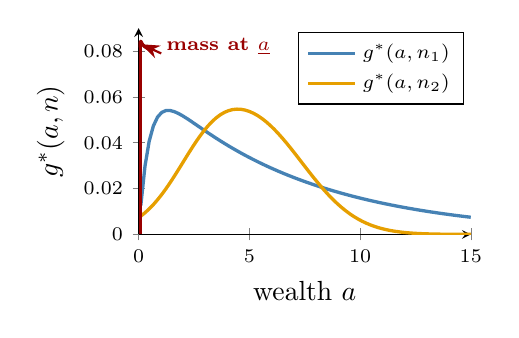
\begin{tikzpicture}
\begin{axis}[
    width=5.8cm, height=4.2cm,
    xlabel={wealth $a$}, ylabel={$g^*(a,n)$},
    xmin=0, xmax=15, ymin=0, ymax=0.09,
    axis lines=left,
    scaled y ticks=false,
    ytick={0,0.02,0.04,0.06,0.08},
    yticklabels={0,0.02,0.04,0.06,0.08},
    tick label style={font=\scriptsize},
    label style={font=\normalsize},
    legend style={at={(0.98,0.98)}, anchor=north east, font=\scriptsize},
]
% Low income state - peaked at low wealth
\addplot[softblue, very thick, domain=0.1:15, samples=80]
    {0.07*exp(-0.15*(x-0.1)) * (1 - exp(-2*x))};
\addlegendentry{$g^*(a, n_1)$}
% High income state - spread to higher wealth
\addplot[softorange, very thick, domain=0.1:15, samples=80]
    {0.05*exp(-(x-5)^2/12) + 0.01*exp(-(x-3)^2/4)};
\addlegendentry{$g^*(a, n_2)$}
% Mass point arrow at borrowing constraint
\draw[harvardcrimson, very thick, ->] (axis cs:0.1,0) -- (axis cs:0.1,0.085);
\node[font=\scriptsize\bfseries, harvardcrimson, fill=white, inner sep=1pt, anchor=west]
    at (axis cs:1.1,0.082) {mass at $\ubar{a}$};
\draw[harvardcrimson, thick, -Stealth] (axis cs:1.02,0.079) -- (axis cs:0.12,0.083);
\end{axis}
\end{tikzpicture}
\end{center}
\end{columns}
\end{frame}

\begin{frame}{Deriving the HJB: Five Steps}
\small
\textbf{Step 1} --- \emphc{Dynamic Programming Principle}. For small $h > 0$:
\[
V(a,n) = \max_c \left\{\int_0^h e^{-\rho t}u(c_t)\ud t + e^{-\rho h}\,\E{V(a_h, n_h) \mid a_0=a, n_0=n}\right\}
\]

\textbf{Step 2} --- \emphc{It\^o's lemma} on $V(a_t, n_t)$ (between jumps of $n$):
\[
dV = V'(a,n)\cdot s(c,a,n)\ud t
\]
(no diffusion term since $da = s\ud t$ is deterministic between jumps)

\textbf{Step 3} --- \emphc{Take expectations}, account for Poisson jumps:
\[
\E{dV} = \left[V'(a,n)\cdot s + \lambda(n)\big(V(a,\hat{n}) - V(a,n)\big)\right]\ud t
\]

\textbf{Step 4} --- \emphc{Substitute} into DPP, divide by $h$, let $h \to 0$:

\textbf{Step 5} --- \emphc{Impose optimality} over $c$:
\[
\boxed{\rho V(a,n) = \max_c\left\{u(c) + V'(a,n)\cdot(wn + ra - c) + \lambda(n)\big(V(a,\hat{n}) - V(a,n)\big)\right\}}
\]
\end{frame}

\begin{frame}{The HJB Equation: Interpretation}
\[
\rho V(a,n) = \max_c\Big\{u(c) + \underbrace{V'(a,n)\cdot s(a,n,c)}_{\text{marginal value $\times$ savings}} + \underbrace{\lambda(n)\big(V(a,\hat{n}) - V(a,n)\big)}_{\text{expected change from income switch}}\Big\}
\]

\vspace{0.2em}
\textbf{Interpretation} (``required return on the value function''):
\begin{itemize}\itemsep2pt
    \item \emphc{LHS}: $\rho V$ = ``required return'' = discount rate $\times$ asset value
    \item \emphc{RHS}: ``dividend'' + ``capital gain'' = total return
    \begin{itemize}
        \item $u(c)$: flow utility (``dividend'')
        \item $V'(a,n) \cdot s$: expected capital gain from saving
        \item $\lambda(n)(V(\hat{n}) - V(n))$: expected gain/loss from income switch
    \end{itemize}
\end{itemize}

\vspace{0.2em}
\begin{center}
\colorbox{uzhgreylight}{\parbox{0.6\textwidth}{\centering\small
The HJB is an \emphc{asset pricing equation}:\\
the value function is priced like a financial asset.}}
\end{center}
\end{frame}

\begin{frame}{Optimal Policy: The Consumption Function}
\small
\textbf{First-order condition} (differentiate HJB w.r.t.\ $c$):
\[
u'(c^*) = V'(a,n) \qquad\Longleftrightarrow\qquad \boxed{c^*(a,n) = (u')^{-1}\!\big(V'(a,n)\big)}
\]

For CRRA utility $u(c) = \frac{c^{1-\gamma}}{1-\gamma}$ with $u'(c) = c^{-\gamma}$:
\[
c^*(a,n) = \left[V'(a,n)\right]^{-1/\gamma}
\]

\vspace{0.1em}
\textbf{Savings function}:
\[
s(a,n) = wn + ra - c^*(a,n)
\]

\vspace{0.1em}
\textbf{State constraint at }$a=\ubar{a}$:
\[
\begin{aligned}
&0<c^*(\ubar a,n)\le wn+r\ubar a,\\
&c^*(\ubar a,n)=\min\{[V_a(\ubar a,n)]^{-1/\gamma},\,wn+r\ubar a\},\\
&s(\ubar a,n)=wn+r\ubar a-c^*(\ubar a,n)\ge 0.
\end{aligned}
\]
{\scriptsize Interior: $u'(c^*)=V_a$. Boundary: constrain consumption so wealth cannot drift below $\ubar a$.}
\end{frame}

\begin{frame}{The Coupled HJB--KFE System}
\begin{center}
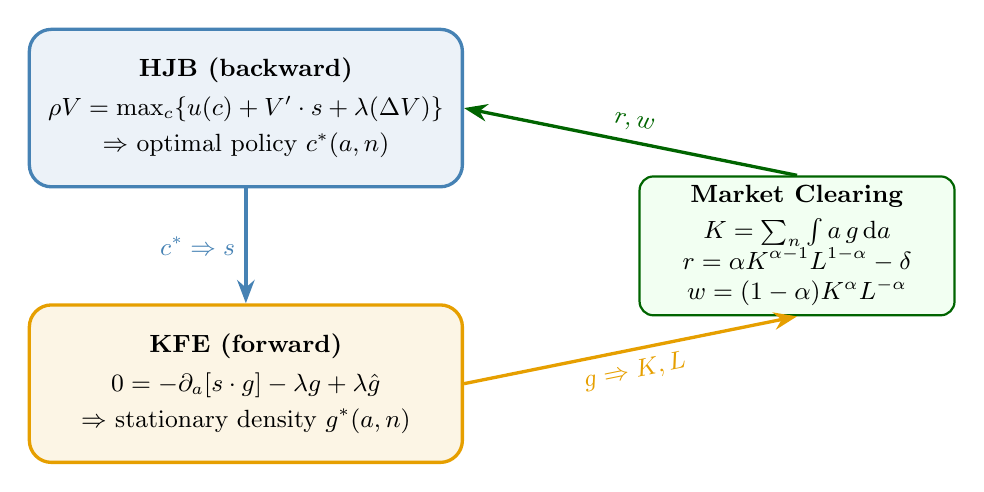
\begin{tikzpicture}[
    box/.style={rectangle, rounded corners=8pt, draw, very thick, minimum width=5.5cm, minimum height=2cm, align=center, font=\small},
    pricebox/.style={rectangle, rounded corners=5pt, draw=darkgreen, thick, fill=green!5, minimum width=4cm, minimum height=1cm, align=center, font=\small},
    arrow/.style={-Stealth, very thick}
]
\node[box, fill=softblue!10, draw=softblue] (hjb) at (0,2.5) {\textbf{HJB (backward)}\\[3pt]
    $\rho V = \max_c\{u(c) + V'\cdot s + \lambda(\Delta V)\}$\\[2pt]
    $\Rightarrow$ optimal policy $c^*(a,n)$};

\node[box, fill=softorange!10, draw=softorange] (kfe) at (0,-1) {\textbf{KFE (forward)}\\[3pt]
    $0 = -\partial_a[s\cdot g] - \lambda g + \lambda \hat{g}$\\[2pt]
    $\Rightarrow$ stationary density $g^*(a,n)$};

\node[pricebox] (mc) at (7,0.75) {\textbf{Market Clearing}\\[2pt]
    $K = \sum_n\int a\,g\ud a$\\
    $r = \alpha K^{\alpha-1}L^{1-\alpha} - \delta$\\
    $w = (1-\alpha)K^\alpha L^{-\alpha}$};

\draw[arrow, softblue] (hjb.south) -- node[left, font=\small] {$c^* \Rightarrow s$} (kfe.north);
\draw[arrow, softorange] (kfe.east) -- node[below, font=\small, sloped] {$g \Rightarrow K, L$} (mc.south);
\draw[arrow, darkgreen] (mc.north) -- node[above, font=\small, sloped] {$r, w$} (hjb.east);
\end{tikzpicture}
\end{center}

\vspace{0.1em}
\textbf{Solution method}: iterate until convergence (Aiyagari, no aggregate shocks):
\begin{enumerate}\itemsep1pt
    \item Guess $r$ $\to$ solve HJB for $V, c^*$ $\to$ solve KFE for $g^*$ $\to$ compute $K$ $\to$ update $r$
\end{enumerate}
\end{frame}

\begin{frame}{Aiyagari (1994): Formal Stationary PDE System}
\footnotesize
\textbf{Production side} (no aggregate shocks):
\[
Y=K^\alpha L^{1-\alpha},\qquad
r=\alpha K^{\alpha-1}L^{1-\alpha}-\delta,\qquad
w=(1-\alpha)K^\alpha L^{-\alpha}.
\]

\vspace{0.1em}
\textbf{Household problem}:
\[
\max_{\{c_t\}} \E{}\!\left[\int_0^\infty e^{-\rho t}u(c_t)\ud t\right],\qquad
da_t=(w z_t+r a_t-c_t)\ud t,\qquad a_t\ge \ubar a,\quad z_t\in\{z_1,z_2\}.
\]

\vspace{0.1em}
\textbf{HJB}:
\[
\rho V(a,z)=\max_c\left\{u(c)+V_a(a,z)\,[w z+r a-c]+\lambda(z)\big(V(a,\hat z)-V(a,z)\big)\right\},
\]
\[
u'(c^*)=V_a,\qquad s(a,z):=w z+r a-c^*(a,z).
\]

\vspace{0.1em}
\textbf{KFE} on $(\ubar a,\infty)$:
\[
0=-\partial_a\!\big[s(a,z)g^*(a,z)\big]-\lambda(z)g^*(a,z)+\lambda(\hat z)g^*(a,\hat z).
\]

\vspace{0.1em}
\textbf{Market clearing \& normalization:}
\[
K=\sum_{z}\int_{\ubar a}^{\infty} a\,g^*(a,z)\ud a,\qquad
L=\sum_{z}\int_{\ubar a}^{\infty} z\,g^*(a,z)\ud a,\qquad
\sum_{z}\int_{\ubar a}^{\infty} g^*(a,z)\ud a=1.
\]
Unknowns: $(V,g^*,r,w,K)$ (or $(V,g^*,r)$ with $w=w(r)$).
\end{frame}

\begin{frame}{Huggett vs.\ Aiyagari: Key Differences}
\small
\begin{center}
\renewcommand{\arraystretch}{1.1}
\begin{tabular}{lcc}
\toprule
& \textbf{Huggett (1993)} & \textbf{Aiyagari (1994)} \\
\midrule
Economy & Endowment & Production ($Y = K^\alpha L^{1-\alpha}$) \\
Asset & Bond $b$ & Capital claim $a$ \\
Supply & Zero net ($\int b = 0$) & Positive ($\int a = K > 0$) \\
Price & Bond return $q$ & Interest rate $r$, wage $w$ \\
Clearing & $\int b\,g\ud b = 0$ & $\int a\,g\ud a = K(r)$ \\
\bottomrule
\end{tabular}
\end{center}

\vspace{0.1em}
\textbf{How the distributions differ:}
\begin{columns}[T]
\column{0.48\textwidth}
\textbf{Huggett:}
\begin{itemize}\itemsep0pt
    \item Wealth centered around $0$ (zero net supply)
    \item Large mass at borrowing constraint
    \item Symmetric-ish with constrained left tail
\end{itemize}

\column{0.48\textwidth}
\textbf{Aiyagari:}
\begin{itemize}\itemsep0pt
    \item Wealth shifted right ($K > 0$)
    \item Long right tail (wealthy agents)
    \item Smaller mass at constraint
\end{itemize}
\end{columns}
\end{frame}

\begin{frame}{The Master Equation}
\footnotesize
\emphc{Key idea}: Substitute KFE, market clearing, and belief consistency \emphc{into} the HJBE.
Result: \emphc{one PDE} characterizing the equilibrium value function:

\vspace{0.1em}
\begin{block}{Master Equation}
\footnotesize
\vspace{-0.2em}
\begin{multline*}
0 = -\rho V(a,n,z,g) + u(c^*) + V_a\,[w(z,g)n+r(z,g)a-c^*] \\
+ \lambda(n)\!\left(V(a,\hat n,z,g)-V(a,n,z,g)\right)
+ V_z\,\mu^z(z) + \tfrac12(\sigma^z)^2V_{zz} \\
+ \sum_{j\in\{1,2\}}\int_{\ubar a}^{\infty}
\frac{\delta V}{\delta g_j}(a,n,z,g)(y)\,\mu^g_j(y,z,g)\ud y
\;=:\;\mathcal{L}V.
\end{multline*}
\vspace{-0.2em}
\end{block}

where $c^*$ satisfies $u'(c^*) = \partial_a V(a,n,z,g)$.

\vspace{0.2em}
\begin{center}
\colorbox{uzhgreylight}{\parbox{0.6\textwidth}{\centering\small
\textbf{``One equation to rule them all''}\\
HJB + KFE + market clearing = master equation}}
\end{center}
\end{frame}


\section{Numerics: Finite Differences versus PINNs}
\begin{frame}{Finite Differences: The Classical Approach}
\small
\textbf{How have economists traditionally solved these models?}

\vspace{0.2em}
\begin{columns}[T]
\column{0.55\textwidth}
\textbf{Finite difference method} (Achdou et al., 2022):
\begin{enumerate}\itemsep1pt
    \item Discretize wealth $a$ on a grid $\{a_1, \ldots, a_I\}$
    \item Approximate derivatives by finite differences:
    \[
    V'(a_i) \approx \frac{V_{i+1} - V_i}{\Delta a} \quad \text{or} \quad \frac{V_i - V_{i-1}}{\Delta a}
    \]
    \item \emphc{Upwind scheme}: use forward diff.\ when savings $> 0$, backward when $< 0$
    \item Iterate HJB $\to$ policy $\to$ KFE $\to$ aggregates $\to$ prices $\to$ HJB
\end{enumerate}

\column{0.42\textwidth}
\begin{center}
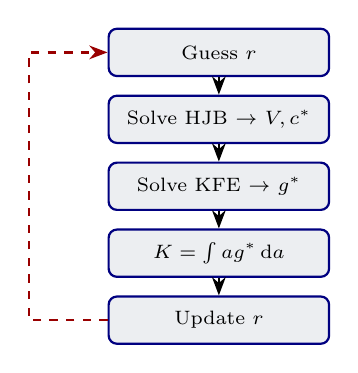
\begin{tikzpicture}[
    box/.style={rectangle, rounded corners=3pt, draw=uzhblue, thick, fill=uzhgreylight, minimum width=2.8cm, minimum height=0.6cm, align=center, font=\scriptsize},
    arrow/.style={-Stealth, thick}
]
\node[box] (guess) at (0,3) {Guess $r$};
\node[box] (hjb) at (0,2.15) {Solve HJB $\to$ $V, c^*$};
\node[box] (kfe) at (0,1.3) {Solve KFE $\to$ $g^*$};
\node[box] (mc) at (0,0.45) {$K = \int ag^*\ud a$};
\node[box] (update) at (0,-0.4) {Update $r$};

\draw[arrow] (guess) -- (hjb);
\draw[arrow] (hjb) -- (kfe);
\draw[arrow] (kfe) -- (mc);
\draw[arrow] (mc) -- (update);
\draw[arrow, dashed, harvardcrimson] (update.west) -- +(-1.0,0) |- (guess.west);
\end{tikzpicture}
\end{center}
\end{columns}

\vspace{0.1em}
{\footnotesize This summarizes the finite-difference workflow; code examples are provided later in Python.}
\end{frame}

\begin{frame}{Finite Differences: What They Produce}
\footnotesize
\begin{columns}[T]
\column{0.48\textwidth}
\textbf{Finite-Difference Example: Aiyagari GE}\\[1pt]
The classical FD approach solves:
\begin{itemize}\itemsep0pt
    \item HJB block: upwind discretization + implicit updates
    \item KFE block: transition operator + stationary distribution
    \item Price block: root-finding for market-clearing $r$
\end{itemize}

\vspace{0.15em}
\textbf{Produces:}
\begin{itemize}\itemsep0pt
    \item Value function $V(a, n)$
    \item Consumption/savings policy $c^*(a, n)$
    \item Stationary density $g^*(a, n)$
    \item Equilibrium prices $r^*, w^*$
\end{itemize}

\vspace{0.15em}
\emphc{This is our ground truth} for validating deep learning methods.

\column{0.48\textwidth}
\begin{center}
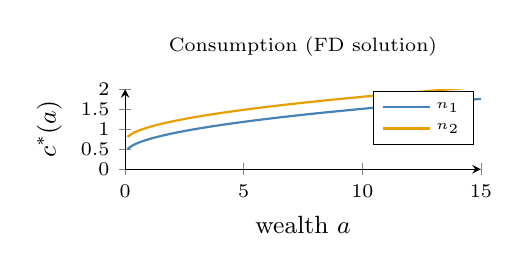
\begin{tikzpicture}
\begin{axis}[
    width=6.1cm, height=2.6cm,
    xlabel={\small wealth $a$}, ylabel={\small $c^*(a)$},
    xmin=0, xmax=15, ymin=0, ymax=2,
    axis lines=left,
    tick label style={font=\scriptsize},
    label style={font=\normalsize},
    title={\scriptsize Consumption (FD solution)},
    title style={at={(0.5,1.08)}},
    legend style={at={(0.98,0.3)}, anchor=south east, font=\tiny},
]
\addplot[softblue, thick, domain=0.1:15, samples=60]
    {0.4 + 0.35*sqrt(x)};
\addlegendentry{$n_1$}
\addplot[softorange, thick, domain=0.1:15, samples=60]
    {0.7 + 0.35*sqrt(x)};
\addlegendentry{$n_2$}
\end{axis}
\end{tikzpicture}

\vspace{0.15em}
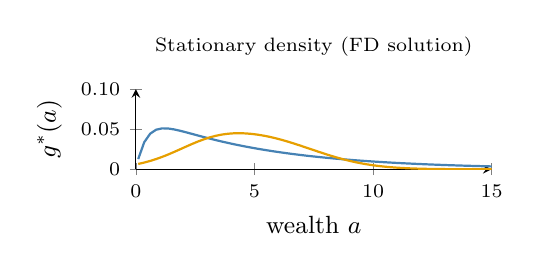
\begin{tikzpicture}
\begin{axis}[
    width=6.1cm, height=2.6cm,
    xlabel={\small wealth $a$}, ylabel={\small $g^*(a)$},
    xmin=0, xmax=15, ymin=0, ymax=0.1,
    axis lines=left,
    scaled y ticks=false,
    ytick={0,0.05,0.10},
    yticklabels={0,0.05,0.10},
    tick label style={font=\scriptsize},
    label style={font=\normalsize},
    title={\scriptsize Stationary density (FD solution)},
    title style={at={(0.5,1.08)}},
]
\addplot[softblue, thick, domain=0.1:15, samples=60]
    {0.07*exp(-0.2*(x-0.1)) * (1 - exp(-2*x))};
\addplot[softorange, thick, domain=0.1:15, samples=60]
    {0.04*exp(-(x-5)^2/12) + 0.01*exp(-(x-3)^2/4)};
\end{axis}
\end{tikzpicture}
\end{center}
\end{columns}
\end{frame}

\begin{frame}{Why Finite Differences Are Not Enough}
\footnotesize
\begin{columns}[T]
\column{0.48\textwidth}
\textbf{FD works well for:}
\begin{itemize}\itemsep1pt
    \item[\textcolor{darkgreen}{\ding{51}}] Stationary HJB--KFE systems
    \item[\textcolor{darkgreen}{\ding{51}}] Low-dimensional states $(a,n)$
    \item[\textcolor{darkgreen}{\ding{51}}] Monotone convergence theory
    \item[\textcolor{darkgreen}{\ding{51}}] Fast sparse linear algebra
\end{itemize}

\column{0.48\textwidth}
\textbf{FD is strained by:}
\begin{itemize}\itemsep1pt
    \item[\textcolor{darkred}{\ding{55}}] Global KS master equation
    \item[\textcolor{darkred}{\ding{55}}] State $(a,n,z,g)$ with distribution $g$
    \item[\textcolor{darkred}{\ding{55}}] Dense tensor-product grids
    \item[\textcolor{darkred}{\ding{55}}] Moment truncation of $g$
\end{itemize}
\end{columns}

\vspace{0.4em}
\begin{alertblock}{Takeaway}
Neural methods do not remove the equilibrium conditions; they approximate
value and distribution maps without building a full grid over $g$.
\end{alertblock}
\end{frame}

\begin{frame}{From Single PDE to Coupled System}
\small
\textbf{Block 1 (PINNs)}: Solve a \emph{single} PDE (Poisson, HJB cake-eating, Black--Scholes).

\vspace{0.2em}
\textbf{Block 2 (this block)}: Solve a \emph{coupled system} of PDEs arising from equilibrium:

\vspace{0.2em}
\begin{center}
\small
\renewcommand{\arraystretch}{1.3}
\begin{tabular}{lll}
\toprule
\textbf{Component} & \textbf{PDE} & \textbf{Unknown} \\
\midrule
HJB (backward) & $\rho V = \max_c\{u(c) + V'\cdot s + \lambda(\Delta V)\}$ & Value $V(a,n)$ \\
KFE (forward) & $0 = -\partial_a[s\cdot g] - \lambda g + \lambda\hat{g}$ & Density $g(a,n)$ \\
Market clearing & $K = \sum_n \int a\,g\ud a$ & Prices $r, w$ \\
\bottomrule
\end{tabular}
\end{center}

\vspace{0.2em}
\textbf{The coupling}: HJB output ($c^* \to s$) is the KFE input (drift).\\
KFE output ($g \to K, L$) determines prices ($r, w$) that enter HJB.

\vspace{0.2em}
\begin{center}
\colorbox{uzhgreylight}{\parbox{0.7\textwidth}{\centering\small
\textbf{PINN approach}: Parameterize \emph{both} $V$ and $g$ by neural networks.\\
Minimize \emph{all} residuals \emphc{jointly} via a single loss function.}}
\end{center}
\end{frame}

\begin{frame}{PINN Architecture for Aiyagari/Huggett}
\small
\begin{columns}[T]
\column{0.55\textwidth}
\textbf{Two neural networks:}
\begin{itemize}\itemsep1pt
    \item $V_\theta(a, n)$: value function network
    \begin{itemize}\itemsep0pt
        \item Input: $(a, n)$ \quad ($n$ encoded as 0/1)
        \item Output: scalar $V$
        \item Architecture: 3--4 hidden layers, 64 neurons, $\tanh$
    \end{itemize}
    \item $g_\phi(a, n)$: density network
    \begin{itemize}\itemsep0pt
        \item Input: $(a, n)$
        \item Output: scalar $g \geq 0$ (use softplus)
        \item Same architecture
    \end{itemize}
\end{itemize}

\vspace{0.2em}
\textbf{Derived quantities} (via auto-diff):
\begin{itemize}\itemsep1pt
    \item $V'_\theta = \partial_a V_\theta$ \quad $\Rightarrow$ consumption: $c^* = (V'_\theta)^{-1/\gamma}$
    \item $\partial_a g_\phi$ \quad $\Rightarrow$ KFE residual
\end{itemize}

\column{0.42\textwidth}
\begin{center}
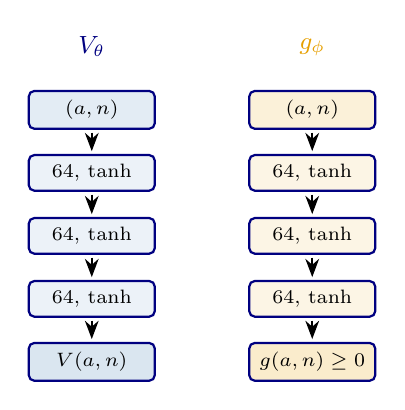
\begin{tikzpicture}[
    layer/.style={rectangle, rounded corners=2pt, draw=uzhblue, thick, minimum width=1.6cm, minimum height=0.4cm, align=center, font=\scriptsize},
    arrow/.style={-Stealth, thick, shorten >=1pt, shorten <=1pt}
]
% Value network
\node[font=\small\bfseries, uzhblue] at (0,4.4) {$V_\theta$};
\node[layer, fill=softblue!15] (v_in) at (0,3.6) {$(a, n)$};
\node[layer, fill=softblue!10] (v_h1) at (0,2.8) {64, $\tanh$};
\node[layer, fill=softblue!10] (v_h2) at (0,2.0) {64, $\tanh$};
\node[layer, fill=softblue!10] (v_h3) at (0,1.2) {64, $\tanh$};
\node[layer, fill=softblue!20] (v_out) at (0,0.4) {$V(a,n)$};

\draw[arrow] (v_in) -- (v_h1);
\draw[arrow] (v_h1) -- (v_h2);
\draw[arrow] (v_h2) -- (v_h3);
\draw[arrow] (v_h3) -- (v_out);

% Density network
\node[font=\small\bfseries, softorange] at (2.8,4.4) {$g_\phi$};
\node[layer, fill=softorange!15] (g_in) at (2.8,3.6) {$(a, n)$};
\node[layer, fill=softorange!10] (g_h1) at (2.8,2.8) {64, $\tanh$};
\node[layer, fill=softorange!10] (g_h2) at (2.8,2.0) {64, $\tanh$};
\node[layer, fill=softorange!10] (g_h3) at (2.8,1.2) {64, $\tanh$};
\node[layer, fill=softorange!20] (g_out) at (2.8,0.4) {$g(a,n) \geq 0$};

\draw[arrow] (g_in) -- (g_h1);
\draw[arrow] (g_h1) -- (g_h2);
\draw[arrow] (g_h2) -- (g_h3);
\draw[arrow] (g_h3) -- (g_out);
\end{tikzpicture}
\end{center}
\end{columns}
\end{frame}

\begin{frame}{Training Algorithm: Jointly Solving HJB + KFE}
\begin{columns}[T]
\column{0.52\textwidth}
\begin{block}{PINN Training (Stationary Equilibrium)}
\footnotesize
\setlength{\itemsep}{0pt}
\begin{algorithmic}[1]
\STATE Initialize $V_\theta$, $g_\phi$, guess $r^{(0)}$ \;\;\textit{(FD reserved for validation)}
\FOR{$k = 1, \ldots, N_{\text{epochs}}$}
    \STATE Sample $M$ collocation points $\{(a_m, n_m)\}$
    \STATE Compute $c_m^* = (V'_\theta(a_m))^{-1/\gamma}$
    \STATE Compute $R_{\text{HJB}}^m$, $R_{\text{KFE}}^m$ via auto-diff
    \STATE Integrate KFE on a fixed asset grid
    \STATE Compute $\mathcal{L}_{\text{SC}}, \mathcal{L}_{\text{flux}}, \mathcal{L}_{\text{mass}}, \mathcal{L}_{\text{MC}}$
    \STATE Total loss: $\mathcal{L} = \sum \kappa_i \mathcal{L}_i$;\; update $\theta,\phi$ (Adam)
    \IF{$k \mod N_r = 0$}
        \STATE $r \leftarrow r + \eta(K^s - K^d)$
    \ENDIF
\ENDFOR
\STATE Freeze collocation grid; run FP64 L-BFGS polish
\end{algorithmic}
\end{block}

\column{0.45\textwidth}
\footnotesize
\textbf{Key choices:}
\begin{itemize}\itemsep0pt
    \item \textbf{Collocation}: sample $(a,n)$ uniformly on $[\ubar{a}, \bar{a}] \times \{n_1, n_2\}$
    \item \textbf{Price update}: update $r$ slowly (every $N_r$ steps) to let NN adapt
    \item \textbf{Loss weights}: start with $\kappa_{\text{HJB}}=\kappa_{\text{KFE}}=1$, larger $\kappa_{\text{SC}},\kappa_{\text{flux}},\kappa_{\text{MC}}$
    \item \textbf{Optimizer}: Adam, lr $\sim 10^{-3}$, then FP64 L-BFGS
    \item \textbf{Validation}: compare against FD only after training
\end{itemize}

\vspace{0.15em}
\begin{center}
\colorbox{uzhgreylight}{\parbox{0.95\columnwidth}{\centering\scriptsize
Same philosophy as Day~5: \emphc{economic equations = loss function};
\emphc{auto-diff = all derivatives}.}}
\end{center}
\end{columns}
\end{frame}

\begin{frame}[shrink=2]{Results: Aiyagari Model (No Aggregate Shocks)}
\small
\textbf{Validation}: Compare EMINN solutions against finite-difference benchmark.

\vspace{0.1em}
\begin{columns}[T]
\column{0.50\textwidth}
\begin{center}
\footnotesize
\renewcommand{\arraystretch}{1.1}
\begin{tabular}{lcc}
\toprule
\textbf{Method} & \textbf{ME Loss} & \textbf{MSE(NN,FD)} \\
\midrule
Finite Pop.\ NN & $3.1 \times 10^{-5}$ & $4.8 \times 10^{-5}$ \\
Discrete State NN & $9.3 \times 10^{-6}$ & $6.6 \times 10^{-5}$ \\
\bottomrule
\end{tabular}
\end{center}

\vspace{0.1em}
\begin{itemize}\itemsep0pt
    \item ME residual: $\sim 10^{-5}$ (excellent)
    \item Agreement with FD: $\sim 10^{-5}$ MSE
    \item Both approaches match FD closely
    \item Consistent across multiple runs
\end{itemize}

\column{0.47\textwidth}
\begin{center}
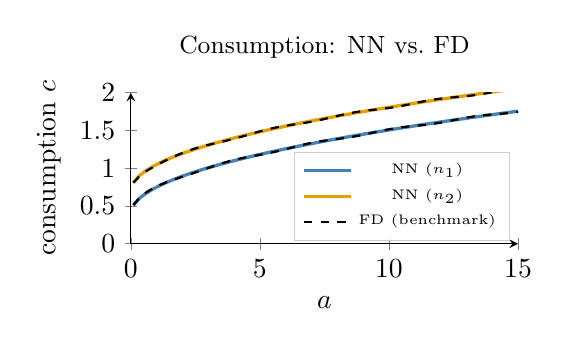
\begin{tikzpicture}
\begin{axis}[
    width=6.5cm, height=3.5cm,
    xlabel={$a$}, ylabel={consumption $c$},
    xmin=0, xmax=15, ymin=0, ymax=2,
    axis lines=left,
    legend style={at={(0.98,0.02)}, anchor=south east, font=\tiny,
                  fill=white, fill opacity=0.85, draw=gray!40, text opacity=1},
    title={\small Consumption: NN vs.\ FD},
    title style={at={(0.5,1.05)}, font=\small},
]
% NN solution
\addplot[softblue, very thick, domain=0.1:15, samples=60]
    {0.4 + 0.35*sqrt(x)};
\addlegendentry{NN ($n_1$)}
\addplot[softorange, very thick, domain=0.1:15, samples=60]
    {0.7 + 0.35*sqrt(x)};
\addlegendentry{NN ($n_2$)}
% FD solution
\addplot[black, thick, dashed, domain=0.1:15, samples=60]
    {0.4 + 0.35*sqrt(x) + 0.01*sin(deg(2*x))};
\addlegendentry{FD (benchmark)}
\addplot[black, thick, dashed, domain=0.1:15, samples=60]
    {0.7 + 0.35*sqrt(x) - 0.01*sin(deg(2*x))};
\end{axis}
\end{tikzpicture}
\end{center}
\end{columns}
\end{frame}

\begin{frame}{Why PINNs over Finite Differences?}
\small
For stationary problems (Huggett/Aiyagari without aggregate shocks):

\vspace{0.1em}
\begin{center}
\footnotesize
\renewcommand{\arraystretch}{1.05}
\begin{tabular}{lcc}
\toprule
& \textbf{Finite Differences} & \textbf{PINN} \\
\midrule
Grid required & Yes ($I$ points) & \emphc{No} (collocation) \\
Upwind scheme & Manual implementation & Auto-diff handles it \\
Curse of dimensionality & $O(I^d)$ & $O(M \cdot |\theta|)$ \\
Extension to higher dim & Very hard & Natural \\
Borrowing constraint & Special treatment & Soft penalty / hard BC \\
Accuracy (2D) & $\sim 10^{-6}$ & $\sim 10^{-4}$ \\
Speed (2D) & Faster & Slower \\
\bottomrule
\end{tabular}
\end{center}

\vspace{0.1em}
\textbf{Verdict}: \textbf{\emph{FD is faster and more accurate}} for low-dim stationary problems --- use it as the gold-standard benchmark. PINNs \emphc{scale to high dimensions}: aggregate shocks (KS, state $\ni g$), multiple assets, richer heterogeneity.
\vspace{-0.2em}

$\Longrightarrow$ Part III: \textbf{EMINNs} for the master equation.
\end{frame}

\begin{frame}{Method Comparison: FD vs.\ PINN vs.\ EMINN}
\footnotesize
\begin{center}
\scriptsize
\renewcommand{\arraystretch}{1.12}
\begin{tabular}{lccc}
\toprule
& \textbf{Finite Diff.} & \textbf{PINN} & \textbf{EMINN} \\
\midrule
Global master eq. & \textcolor{darkred}{\ding{55}} & \textcolor{darkred}{\ding{55}} & \textcolor{darkgreen}{\ding{51}} \\
Stationary equilibrium & \textcolor{darkgreen}{\ding{51}} & \textcolor{darkgreen}{\ding{51}} & \textcolor{darkgreen}{\ding{51}} \\
Grid required & Yes & No & No \\
High-dimensional scaling & Limited & Better, validate & Better, validate \\
Handles $g$ as state & Standard: no & No & Via $\hat{\varphi}$ \\
Theory & Strong in low dim & Limited & Limited \\
Low-dim accuracy & $\sim 10^{-6}$ & problem-dependent & reported $\sim 10^{-5}$ \\
\bottomrule
\end{tabular}
\end{center}

\vspace{0.1em}
\textbf{Bottom line:}
\begin{itemize}\itemsep0pt
    \item \textbf{Stationary, low-dim}: FD is fast and reliable. Use it as benchmark.
    \item \textbf{Aggregate shocks}: EMINNs target global master-equation solutions.
    \item \textbf{PINNs}: useful bridge for the coupled HJB--KFE system.
\end{itemize}
\end{frame}

\begin{frame}{Code Companion: Run This Live}
\footnotesize
\textbf{Day 6 companion notebooks (self-contained, PyTorch):}
\begin{itemize}\itemsep2pt
    \item \textbf{NB 06} \textit{(self-study)}: \texttt{06\_PE\_Discrete\_HJB\_PINN.ipynb} --- 1D PE with discrete income: upwind FD + PINN
    \item \textbf{NB 07} \textit{(self-study)}: \texttt{07\_PE\_Diffusion\_HJB\_PINN.ipynb} --- 2D PE with OU earnings: 2D FD + PINN
    \item \textbf{NB 08} \textit{(in-class)}: \texttt{08\_Aiyagari\_Continuous\_Time\_FD\_and\_PINN\_PyTorch.ipynb} --- full GE Aiyagari: HJB + KFE + market clearing
\end{itemize}

\vspace{0.2em}
\textbf{Suggested in-class demo flow:}
\begin{enumerate}\itemsep1pt
    \item Start with NB~06 (simplest, self-study): FD convergence, then PINN overlay
    \item Move to NB~07 (self-study): 2D contour plots, cross-sections, mesh-free advantage
    \item Focus on NB~08 (in-class): full GE loop, PINN vs FD agreement diagnostics
\end{enumerate}
\end{frame}


\end{document}
